\documentclass{article}
%http://tex.stackexchange.com/a/196456/7712
\usepackage{tikz,etoolbox}
\usetikzlibrary{calc}
\makeatletter
\newcounter{tikzline}
\def\lines{1,2,3}

\begin{document}

  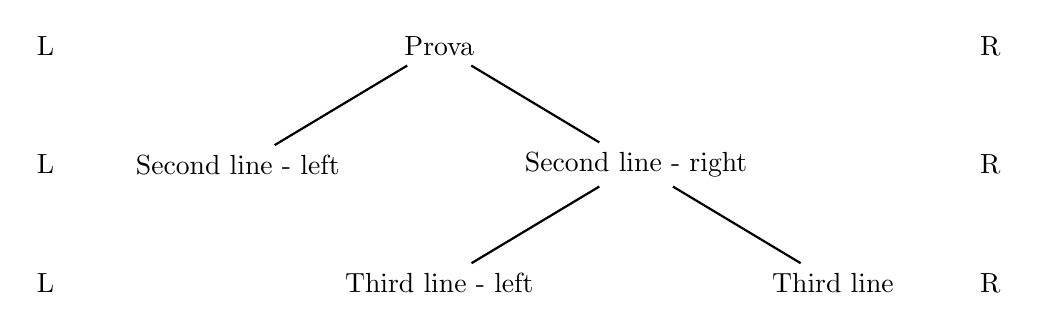
\begin{tikzpicture}[sibling distance=5cm,
                      edge from parent/.style={draw,thick,-}]
   \node(1){Prova}
        child {node[align=left] {Second line - left } }
        child {node(2)[align=right] {Second line - right}
            child {node (3)[align=left] { Third line - left}}
            child {node {Third line }}
        };


  % loop over the "left" nodes
  \foreach \Node in \lines {%\y1=y-coord of the node
    \path let \p1=($ (\Node) $) in node at (-5,\y1){L};
  }

  % loop over the "right" nodes
  \foreach \Node in \lines {%\y1=y-coord of the node
    \path let \p1=($ (\Node) $) in node at (7,\y1){R};
  }

\end{tikzpicture}

\end{document}